\subsubsection{11.12.14}

\begin{enumerate}
	\item The time of beginning and ending of the meeting: 17:30 - 23:30
	\item Purposes of the meeting:
	\begin{enumerate}
		\item To finish installation of steel crossbar on the lift.
		
		\item To add second servo on the MOB.
		
		\item To package the robot for transportation it to competition "Robofest-Ryazan".
	\end{enumerate}
	\item Work that has been done:
	\begin{enumerate}
		\item It was installed another one crossbar. It was decided to leave aluminium axis with the tube on the bottom crossbar because steel axis can't get into the tube. In addition aluminium axis doesn't bend due to the tube. Also the tube reduces the friction becaise it can rotate on the axis.
		
		\item The aluminium axis with the tube was oiled for additional redusing the friction.
		
		\begin{figure}[H]
			\begin{minipage}[h]{0.2\linewidth}
				\center  
			\end{minipage}
			\begin{minipage}[h]{0.6\linewidth}
				\center{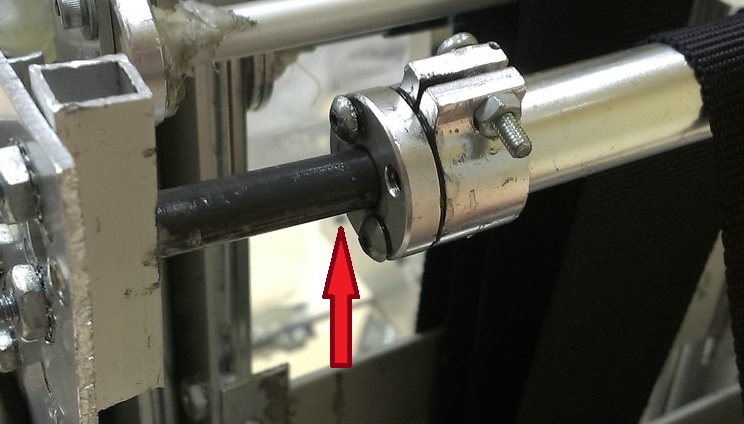
\includegraphics[scale=0.3]{days/11.12.14/images/01}}
				\caption{The bottom crossbar was oiled}
			\end{minipage}
		\end{figure}
		
		\item Two servos can't to overturn the bucket. So it was decided to return MOB to the previous position (in the center part of the top slat).
		
		\item Robot was packaged for transportation.
		
	\end{enumerate}
	\item Results: 
	\begin{enumerate}
		\item Steel crossbars were installed.
		
		\item It was decided to move MOB to the previous position.
		
		\item MOB wasn't moved.
		
	\end{enumerate}
	\item Tasks for the next meetings:
	\begin{enumerate}	
		\item To move MOB to the previous position.
		
		\item To train on the control of the robot.
		
		\item To install mechanism that will direct balls vertically.
		
	\end{enumerate}
\end{enumerate}
\fillpage